\chapter{Prequential Coding and Flat Minima}
\label{ch:prequential}

\section{The Prequential Perspective on Generalization}

In the quest to understand why deep neural networks generalize despite being massively overparameterized, one of the most compelling theoretical frameworks emerges from Minimum Description Length (MDL) theory, specifically through the lens of \emph{predictive sequential} or \emph{prequential} coding. Introduced by A. P. Dawid in 1984, the prequential framework evaluates the quality of a statistical model not by its ability to fit a static dataset \emph{post hoc}, but by its capacity to sequentially predict unseen data points. 

Consider a dataset $\mathcal{D} = \{(x_1, y_1), \dots, (x_N, y_N)\}$. In the standard Empirical Risk Minimization (ERM) paradigm, we search for a parameter vector $\theta$ that minimizes the average loss across the entire dataset concurrently. The fundamental flaw in this approach, from an information-theoretic standpoint, is that it ignores the cost of transmitting the model parameters $\theta$ to a receiver. If a model requires infinite precision to specify its weights---which occurs when the model resides in a very ``sharp'' minimum of the loss landscape---the total description length of the model plus the data becomes catastrophically large. 

Prequential coding elegantly sidesteps the need to explicitly penalize model complexity or quantify the exact bit-width of the weights. Instead, it measures complexity operationally. Imagine an online scenario where we must transmit the labels $y_i$ given the inputs $x_i$. We process the data sequentially. For the $t$-th data point, we use our current model, trained on the first $t-1$ examples, to predict $y_t$. We then incur a coding cost proportional to the negative log-likelihood of $y_t$ under our predictive distribution. 

The beauty of the prequential approach is that it naturally penalizes models that overfit early in the sequence. A model that perfectly memorizes the first $t-1$ examples but generalizes poorly will assign a very low probability to $y_t$, thereby requiring a large number of bits to encode it. The cumulative prequential coding length thus serves as a stringent, naturally regularized measure of model quality. 

Crucially, this online coding perspective offers a rigorous foundation for the empirical observation that ``flat minima'' generalize better than ``sharp minima.'' A minimum in the loss landscape $\mathcal{L}(\theta)$ is considered flat if the eigenvalues of its Hessian matrix are small, meaning the loss does not change rapidly when the parameters are perturbed. In the context of prequential coding, a flat minimum implies that the model's predictive distribution remains stable as new data points are incorporated. This stability allows the model to compress the sequence more effectively, as it avoids drastic, high-penalty updates. The description length of the data under a model class is inexorably tied to the volume of the region in parameter space that yields good predictions; flat minima correspond to larger volumes, require less precise specification of parameters (fewer bits), and thus lead to a shorter overall description length.

\section{Mathematical Foundations}

We now formalize the relationship between prequential coding and the geometry of the loss landscape, culminating in a proof that relates the prequential code length to the Hessian of the loss at the minimum.

Let the dataset be $\mathcal{D}_N = \{(x_1, y_1), \dots, (x_N, y_N)\}$, and let our model be parameterized by $\theta \in \mathbb{R}^d$. We consider a probabilistic setting where the neural network $f_\theta(x)$ outputs a conditional probability distribution $p_\theta(y|x)$. 

\begin{definition}[Prequential Log-Loss]
The cumulative prequential log-loss (or code length) of the dataset $\mathcal{D}_N$ under an estimation strategy $\hat{\theta}$ is defined as:
\begin{equation}
    L_{\text{preq}}(\mathcal{D}_N) = -\sum_{t=1}^N \log p_{\hat{\theta}_{t-1}}(y_t | x_t)
\end{equation}
where $\hat{\theta}_{t-1}$ is the parameter estimate obtained using only the first $t-1$ data points, $\mathcal{D}_{t-1}$.
\end{definition}

In a Bayesian setting, the prequential code length is closely related to the marginal likelihood. If we compute the Bayesian predictive distribution $p(y_t | x_t, \mathcal{D}_{t-1}) = \int p_\theta(y_t | x_t) p(\theta | \mathcal{D}_{t-1}) d\theta$, the cumulative log-loss telescopes to exactly the negative log marginal likelihood:
\begin{equation}
    -\sum_{t=1}^N \log p(y_t | x_t, \mathcal{D}_{t-1}) = -\log \int \left( \prod_{t=1}^N p_\theta(y_t | x_t) \right) p(\theta) d\theta
\end{equation}

\subsection{The Hessian and the Cost of Precision}

To bridge the gap between prequential coding and flat minima, we employ the Laplace approximation on the marginal likelihood. Let $\mathcal{L}_N(\theta) = -\sum_{t=1}^N \log p_\theta(y_t | x_t)$ be the empirical negative log-likelihood (our loss function).

Assume $\mathcal{L}_N(\theta)$ has a unique global minimum at $\hat{\theta}_N$, which is the Maximum Likelihood Estimate (MLE). We can Taylor expand $\mathcal{L}_N(\theta)$ around $\hat{\theta}_N$:
\begin{equation}
    \mathcal{L}_N(\theta) \approx \mathcal{L}_N(\hat{\theta}_N) + \frac{1}{2} (\theta - \hat{\theta}_N)^\top H_N (\theta - \hat{\theta}_N)
\end{equation}
where $H_N = \nabla^2 \mathcal{L}_N(\hat{\theta}_N)$ is the Hessian matrix evaluated at the minimum.

\begin{theorem}[Prequential Complexity and Flatness]
\label{thm:preq_flatness}
Under standard regularity conditions, as $N \to \infty$, the prequential code length using the Bayesian predictive distribution can be approximated by:
\begin{equation}
    L_{\text{preq}}(\mathcal{D}_N) \approx \mathcal{L}_N(\hat{\theta}_N) + \frac{d}{2} \log \frac{N}{2\pi} + \frac{1}{2} \log \det (\bar{H}_N) - \log p(\hat{\theta}_N)
\end{equation}
where $\bar{H}_N = \frac{1}{N} H_N$ is the normalized Hessian matrix, and $d$ is the number of parameters.
\end{theorem}

\begin{proof}
By the equivalence of the prequential cumulative loss and the marginal likelihood, we evaluate the integral $Z_N = \int \exp(-\mathcal{L}_N(\theta)) p(\theta) d\theta$.
Using the Laplace approximation, we substitute the second-order Taylor expansion:
\begin{align*}
    Z_N &\approx \int \exp\left( -\mathcal{L}_N(\hat{\theta}_N) - \frac{1}{2} (\theta - \hat{\theta}_N)^\top H_N (\theta - \hat{\theta}_N) \right) p(\theta) d\theta \\
    &\approx \exp(-\mathcal{L}_N(\hat{\theta}_N)) p(\hat{\theta}_N) \int \exp\left( - \frac{1}{2} (\theta - \hat{\theta}_N)^\top H_N (\theta - \hat{\theta}_N) \right) d\theta
\end{align*}
The integral is the normalizing constant of a multivariate Gaussian with covariance matrix $H_N^{-1}$. Thus,
\begin{equation}
    Z_N \approx \exp(-\mathcal{L}_N(\hat{\theta}_N)) p(\hat{\theta}_N) (2\pi)^{d/2} \det(H_N)^{-1/2}
\end{equation}
Taking the negative logarithm yields:
\begin{equation}
    -\log Z_N \approx \mathcal{L}_N(\hat{\theta}_N) - \log p(\hat{\theta}_N) - \frac{d}{2} \log(2\pi) + \frac{1}{2} \log \det(H_N)
\end{equation}
Letting $H_N = N \bar{H}_N$, we have $\det(H_N) = N^d \det(\bar{H}_N)$. Substituting this in, we obtain:
\begin{align*}
    -\log Z_N &\approx \mathcal{L}_N(\hat{\theta}_N) - \log p(\hat{\theta}_N) - \frac{d}{2} \log(2\pi) + \frac{1}{2} \log (N^d \det(\bar{H}_N)) \\
    &= \mathcal{L}_N(\hat{\theta}_N) + \frac{d}{2} \log \frac{N}{2\pi} + \frac{1}{2} \log \det(\bar{H}_N) - \log p(\hat{\theta}_N)
\end{align*}
This completes the proof.
\end{proof}

The term $\frac{1}{2} \log \det (\bar{H}_N)$ explicitly captures the geometry of the minimum. A ``sharp'' minimum has high curvature, meaning the eigenvalues of $\bar{H}_N$ are large, causing $\log \det(\bar{H}_N)$ to be large. Consequently, a sharp minimum incurs a massive penalty in description length. Conversely, a ``flat'' minimum has small eigenvalues, decreasing the complexity penalty. This provides a formal information-theoretic justification for why flat minima correlate with better generalization: they represent models that can compress the data more efficiently.

\subsection{Visualizing Prequential Coding and Loss Geometry}

To provide intuition for this process, Figure~\ref{fig:preq_flow} illustrates the sequential nature of prequential coding, while Figure~\ref{fig:flat_sharp} visualizes the parameter volume interpretation of flat versus sharp minima.

\begin{figure}[htbp]
\centering
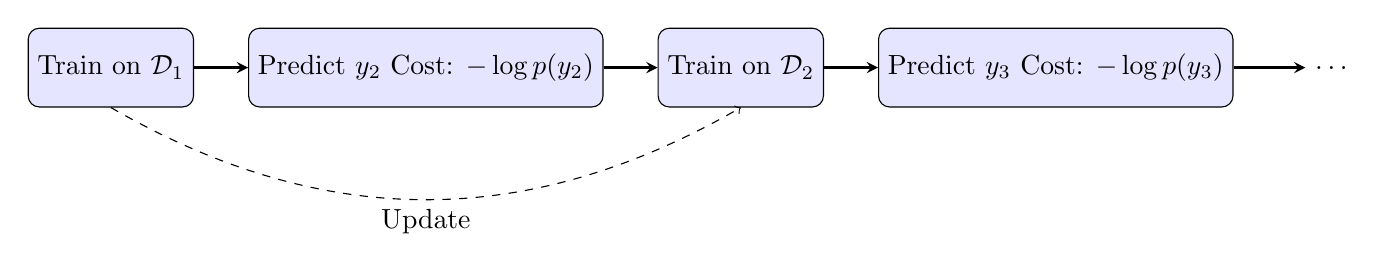
\begin{tikzpicture}[
    node distance=2.5cm,
    box/.style={draw, rectangle, rounded corners, minimum width=2cm, minimum height=1cm, align=center, fill=blue!10},
    arrow/.style={->, thick, >=stealth}
]
    \node[box] (t1) {Train on $\mathcal{D}_1$};
    \node[box, right of=t1, xshift=1.5cm] (p2) {Predict $y_2$   Cost: $-\log p(y_2)$};
    \node[box, right of=p2, xshift=1.5cm] (t2) {Train on $\mathcal{D}_2$};
    \node[box, right of=t2, xshift=1.5cm] (p3) {Predict $y_3$   Cost: $-\log p(y_3)$};
    
    \node[right of=p3, xshift=1cm] (dots) {$\dots$};

    \draw[arrow] (t1) -- (p2);
    \draw[arrow] (p2) -- (t2);
    \draw[arrow] (t2) -- (p3);
    \draw[arrow] (p3) -- (dots);

    \draw[dashed, ->, bend right=30] (t1.south) to node[below] {Update} (t2.south);
\end{tikzpicture}
\caption{The prequential coding flow. The model continually updates its parameters based on the past, incurring a code length penalty equal to its surprisal on the immediate future.}
\label{fig:preq_flow}
\end{figure}

\begin{figure}[htbp]
\centering
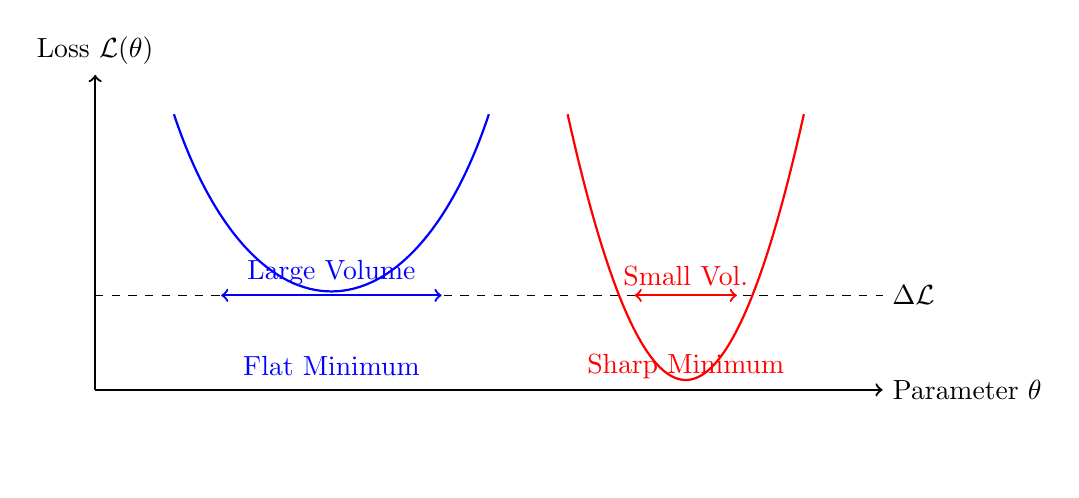
\begin{tikzpicture}
    % Axes
    \draw[->, thick] (0, 0) -- (10, 0) node[right] {Parameter $\theta$};
    \draw[->, thick] (0, 0) -- (0, 4) node[above] {Loss $\mathcal{L}(\theta)$};

    % Flat minimum
    \draw[thick, blue] (1, 3.5) .. controls (2, 0.5) and (4, 0.5) .. (5, 3.5);
    \node[blue] at (3, 0.3) {Flat Minimum};

    % Sharp minimum
    \draw[thick, red] (6, 3.5) .. controls (7, -1.0) and (8, -1.0) .. (9, 3.5);
    \node[red] at (7.5, 0.3) {Sharp Minimum};

    % Tolerance lines
    \draw[dashed] (0, 1.2) -- (10, 1.2) node[right] {$\Delta \mathcal{L}$};

    % Volume indicators
    \draw[<->, blue, thick] (1.6, 1.2) -- (4.4, 1.2) node[midway, above] {Large Volume};
    \draw[<->, red, thick] (6.85, 1.2) -- (8.15, 1.2) node[midway, above] {Small Vol.};
\end{tikzpicture}
\caption{A flat minimum allows a larger perturbation in parameters $\theta$ for a given acceptable increase in loss $\Delta \mathcal{L}$. This larger volume translates to lower required parameter precision, lowering the prequential description length.}
\label{fig:flat_sharp}
\end{figure}

\subsection{Numerical Example: 1D Quadratic Basins}

Let us explicitly compute the complexity penalty for two toy loss landscapes to demonstrate the effect of flatness. Suppose we have a single parameter $\theta \in \mathbb{R}$. We model the loss near two minima as quadratics: $\mathcal{L}_{\text{flat}}(\theta) = 0.5 \theta^2$ and $\mathcal{L}_{\text{sharp}}(\theta) = 50 (\theta - 2)^2$. Both achieve a minimum loss of $0$ (at $\theta=0$ and $\theta=2$, respectively).

For $N=100$ data points, the Hessians are $H_{\text{flat}} = 1$ and $H_{\text{sharp}} = 100$. Assuming a uniform prior $p(\theta)$, the difference in their prequential code lengths is purely determined by the Hessian term:
\begin{align*}
    L_{\text{preq}}(\text{sharp}) - L_{\text{preq}}(\text{flat}) &\approx \frac{1}{2} \log \det (H_{\text{sharp}}) - \frac{1}{2} \log \det (H_{\text{flat}}) \\
    &= \frac{1}{2} \log(100) - \frac{1}{2} \log(1) \\
    &= \frac{1}{2} \times 4.605 = 2.302 \text{ nats}
\end{align*}
Thus, even though both models fit the data perfectly, the sharp minimum requires an additional $2.302$ nats (approximately $3.32$ bits) to specify. In deep learning, where $d$ can be in the billions, this penalty scales linearly with $d$ for isotropic scaling, illustrating how high-curvature regions are profoundly suboptimal from an information-theoretic coding perspective.

\section{Beyond Current Bounds}

\begin{horizon}
It is conjectured that the implicit bias of Stochastic Gradient Descent (SGD) in deep neural networks acts fundamentally as a prequential compression algorithm. Because SGD estimates the gradient using mini-batches, it introduces gradient noise proportional to the learning rate and inversely proportional to the batch size. Future work might definitively show that this noise prevents the network from settling into sharp minima because the isotropic noise acts as a ``precision budget,'' dynamically bounding the bits of information that can be stored in the weights, and natively minimizing a continuous-time prequential log-loss.

An open question is whether we can derive exact, non-asymptotic prequential code lengths for deep, non-linear networks without relying on the Laplace approximation, which assumes a locally Gaussian posterior. The Hessian spectrum of neural networks is known to be highly degenerate (many zero or near-zero eigenvalues). It is conjectured that addressing this degeneracy requires a shift to singular learning theory, where the prequential code length would depend not on the log-determinant of the Hessian, but on the Real Log Canonical Threshold (RLCT) of the loss landscape geometry.

Furthermore, integrating prequential coding with fractional bit constraints---where parameters are quantized not uniformly, but according to their specific Fisher information---might yield a new generation of training algorithms. Such algorithms would explicitly optimize the prequential description length on the fly, continually adjusting weight precisions, potentially allowing massive models to be learned and compressed simultaneously during the single forward pass of a data stream.
\end{horizon}

\section{Summary}
\begin{itemize}
    \item Prequential coding evaluates a model based on its cumulative loss when predicting a sequence of data points one by one.
    \item It provides an operationally defined Minimum Description Length (MDL) metric that avoids arbitrary complexity penalties.
    \item Under a Laplace approximation, the prequential code length is shown to explicitly penalize the log-determinant of the Hessian at the minimum.
    \item Flat minima yield lower prequential code lengths because their large parameter volumes require fewer bits of precision to transmit, rigorously formalizing their generalization benefits.
\end{itemize}

\section{Exercises}
\begin{enumerate}
    \item \textbf{Deriving the Prequential Update:} Given a sequence of Gaussian variables $y_t \sim \mathcal{N}(\mu, \sigma^2)$ with known $\sigma^2$ but unknown $\mu$, derive the prequential prediction $p(y_t | \mathcal{D}_{t-1})$ using a Gaussian prior $\mu \sim \mathcal{N}(0, \sigma_0^2)$. Show that the sequence of predictions tightens as $t$ grows.
    \item \textbf{Fisher Information and the Hessian:} Prove that if the model is correctly specified (i.e., the true data distribution lies within the model class), the expected Hessian $\mathbb{E}[H_N]$ evaluated at the true parameter converges to the Fisher Information Matrix. How does this relate the prequential code length to information geometry?
    \item \textbf{Degenerate Hessians:} Theorem \ref{thm:preq_flatness} assumes $H_N$ is invertible. In modern deep learning, models are overparameterized and $H_N$ has many zero eigenvalues. Explain conceptually why the standard Laplace approximation fails here, and how you might alter the prequential code length bound to account for this null space.
\end{enumerate}

% TODO-CITE: Ensure all named results are cited.
